
\chapter{Detailed Analysis and Comparison of Results}
\label{cha:conclusions_future_directions}
In this chapter we present the benchmark results on different technologies and strategies on the two chose algorithms previously mentioned in previous chapter, as detailed in the preceding chapters. Our investigation spanned various strategies and implementations, culminating in a nuanced understanding of the relative performance and characteristics of different approaches across .NET, Java, and other programming environments. Here, we consolidate these findings, reflecting on their broader implications within the field of asynchronous programming. Furthermore, we outline potential avenues for future research that emerge from our study, paving the way for continued exploration and innovation in this domain.


\section{.NET Benchmarking}
\label{sec:dotnet_implementation}

In this subsection, we focus on the benchmark using different strategies in .NET programming environment.

\subsection{Find the biggest word algorithm results}
\label{subsubsec:biggest_word_results_cs}

For the find the biggest word algorithm, used in C\# implementations are the following strategies:
\begin{itemize}
    \item \textbf{Baseline}: This strategy serves as the basic approach for finding the biggest word and acts as a baseline for comparison using blocking IO to retrieve data from files.
    \item \textbf{Baseline NIO}: This strategy uses a non-blocking IO to retrieve data from files. Each "fileread" is non-blocking, however, there are several tasks running in parallel reading files, the results are only shown when all tasks are finished. 
    \item \textbf{Parallel}: An approach that makes the use of parallelization using blocking IO.
    \item \textbf{AsyncEnumerables}: This approach uses asynchronous programming with enumerable collections.
    \item \textbf{RxNet}: This strategy uses the Reactive Extensions (Rx) library with asynchronous file reading operations.
    \item \textbf{Linq}: This strategy uses Language Integrated Query (LINQ) for finding the biggest word.
\end{itemize}

In the following graphic, we have the results in seconds for each strategy:
\begin{figure}[H]
    \centering
    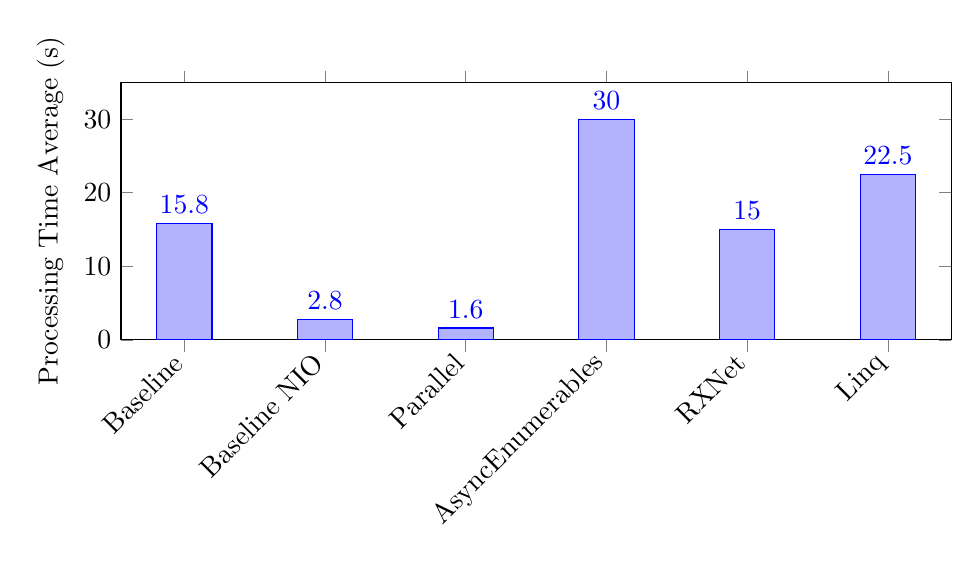
\begin{tikzpicture}
    \begin{axis}[
        ybar=2*\pgflinewidth,
        width=1.0\textwidth,
        height=0.4\textwidth,
        bar width=20pt,
        enlarge x limits={0.09}, % Adjust the value as needed
        enlarge y limits=false, % Ensure only x-limits are enlarged
        legend style={at={(0.5,-0.2)}, anchor=north, legend columns=-1},
        ylabel={Processing Time Average (s)},
        symbolic x coords={Baseline, Baseline NIO, Parallel, AsyncEnumerables, RXNet, Linq},
        xtick=data,
        xticklabel style={rotate=45, anchor=east},
        nodes near coords,
        nodes near coords align={vertical},
        ymin=0, ymax=35,
        ]
    \addplot coordinates {(Baseline, 15.8) (Baseline NIO, 2.8) (Parallel, 1.6) (AsyncEnumerables, 30) (RXNet, 15) (Linq, 22.5)};
    \end{axis}
    \end{tikzpicture}
    \caption{Processing times for different strategies for "Find the biggest word".}
    \label{fig:biggest_word_results_cs_2}
\end{figure}

From these results, it is apparent that the baseline approach using non-blocking IO has an advantage over its blocking counterpart because of the parallelization used in NIO baseline. However, it is also evident that the parallelization with blocking IO solution still holds an advantage over its pipeline competitors.
Taking into account the pipeline technologies, we can see that the overall performance is worse compared to strategies that do not use pipelines. In this context, RxNet demonstrates a performance advantage over both Linq and AsyncEnumerables strategies. It was expected that, since Linq uses a blocking IO source, however, on the other side, Linq solution outperform AsyncEnumerables solution. This may imply that for this particular algorithm, the AsyncEnumerable strategy incurs a higher internal overhead than intended although using non-blocking IO while Linq blocks for each IO operation. 
It's important to reinforce that parallelization has huge advantages although not making use of non-blocking IO.

\subsection{Group Word Results}
\label{subsubsec:group_word_processing_times_cs}
In this subsection, we concentrate on the task of grouping words from a file using different strategies. The strategies that we evaluate here include:
\vspace{-10pt}
\begin{itemize}
    \item \textbf{Baseline}: This strategy serves as the basic approach for word grouping and acts as a baseline for comparison.
    \item \textbf{Linq}: Like in the find word algorithm, this strategy uses Language Integrated Query (LINQ) in a synchronous manner.
    \item \textbf{AsyncEnumerable}: This strategy uses .NET async enumerables to process the asynchronous data .
    \item \textbf{RxNet}: Here, the Reactive Extensions (Rx) library is used to handle data sequences asynchronously and event-based.
\end{itemize}

\begin{figure}[H]
    \centering
    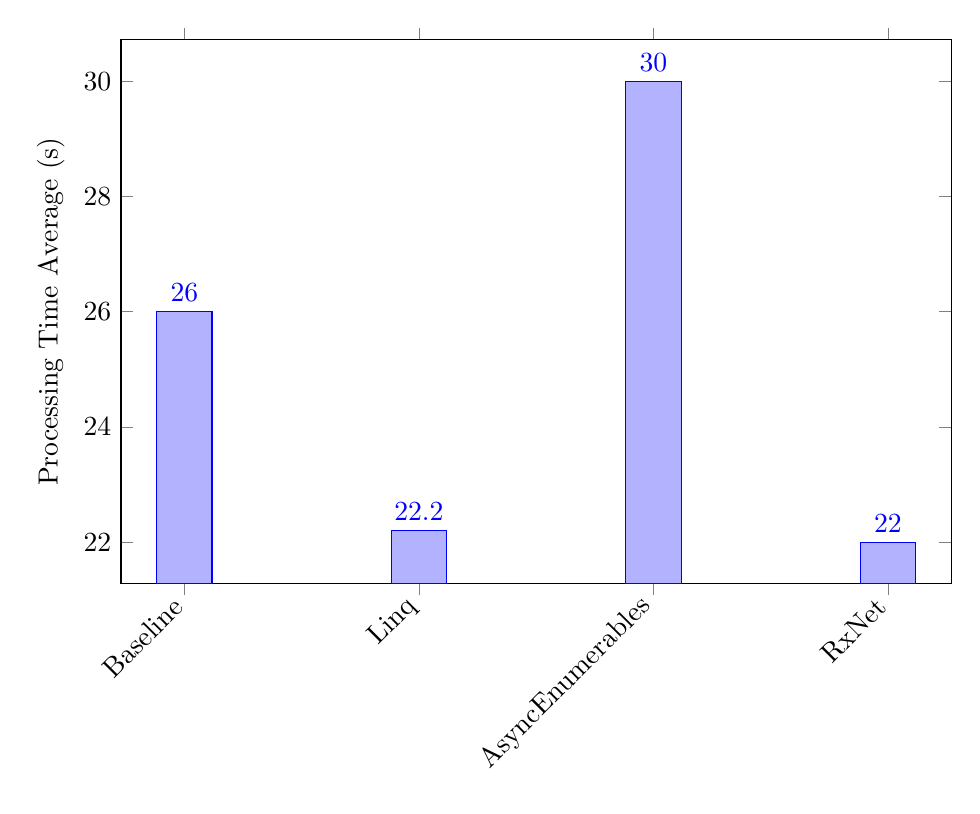
\begin{tikzpicture}
    \begin{axis}[
        ybar=2*\pgflinewidth,
        width=1.0\textwidth,
        height=0.7\textwidth,
        bar width=20pt,
        enlargelimits=0.09,
        legend style={at={(0.5,-0.2)}, anchor=north, legend columns=-1},
        ylabel={Processing Time Average (s)},
        symbolic x coords={Baseline, Linq, AsyncEnumerables, RxNet},
        xtick=data,
        xticklabel style={rotate=45, anchor=east},
        nodes near coords,
        nodes near coords align={vertical},
        ]
    \addplot coordinates {(Baseline, 26.0) (Linq, 22.2) (AsyncEnumerables, 30) (RxNet, 22.0)};
    \end{axis}
    \end{tikzpicture}
    \caption{Processing times for different strategies for "Group Words".}
    \label{fig:group_word_processing_times_cs}
\end{figure}

First of all, its important to make clear once again, that this algorithm is memory-intensive; in this case, it uses dictionaries, to hold information about each word, where the word is the key and the value is number of occurrences for each word repetition in the dataset.
Taking, that in account, and once again as explained, the baseline strategy serves a standard for performance comparison with other solutions. While straightforward, in this case, it does not leverage the advanced features of other approaches, resulting in a moderate processing time. In comparison, the Linq strategy, shows an improvement in performance over the baseline. This suggests that the streamlined querying capabilities of LINQ, despite being synchronous, can efficiently handle the algorithm's requirements better than the baseline approach in this memory-intensive scenario.
On the other hand, the AsyncEnumerable approach, which uses .NET async enumerables to process data asynchronously, exhibits a longer processing time in this context. This indicates that while async enumerables are beneficial for certain applications, their performance in memory-intensive tasks like "Group Words," which heavily relies on dictionaries, might not be optimal.
Furthermore, the RxNet implementation, also demonstrates competitive performance. This underscores the potential of RxNet in efficiently managing asynchronous data flows, especially in scenarios where the processing time is crucial.
In this case, the performance between approaches was very similar, making the choice between blocking and non-blocking I/O operations less significant and harder to draw many conclusions from. However, at first glance, it appears that memory-intensive operations tend to overshadow any potential performance gains from using non-blocking I/O operations. Nevertheless, this assertion can change drastically depending on the project needs.
The results, in this case, indicate that the optimal strategy for such algorithms would depend more on how they handle memory-intensive operations rather than the differences in I/O operation types.

\section{Java/Kotlin Benchmarking}
\label{sec:java_implementation}
In this section, we explore and assess diverse strategies applied in Java and Kotlin to process files, and we scrutinize their performances solving the "Find Word" an "Group Word algorithms"

\subsection{Biggest Word Results}
\label{subsubsec:biggest_word_results}

The strategies used in JAVA are:
\begin{itemize}
    \item \textbf{Baseline}: This strategy illustrates a basic non-blocking I/O operation, serving as a comparison baseline.
    \item \textbf{Flux}: These strategies leverage the Reactor Flux model from Java's Project Reactor library. The former follows a standard non-concurrent processing model, while the latter introduces parallelization for improved performance.
    \item \textbf{RXJava}: This strategy employ the RXJava library. They replace the Reactor Flux with Observables, with the distinction being made between non-concurrent and concurrent processing.
    \item \textbf{Streams and parallelization}: Implementation of three strategies that use Java's Streams API and explore handling of blocking operations under three different conditions: standard usage, raw multithreading using threadpools and using parallel method in the streams API.
    \item \textbf{Flow (Kotlin)}: This strategy utilizes Kotlin's Flow API
\end{itemize}

In the following graphic, we have the results in seconds for each strategy:
\begin{figure}[H]
    \centering
    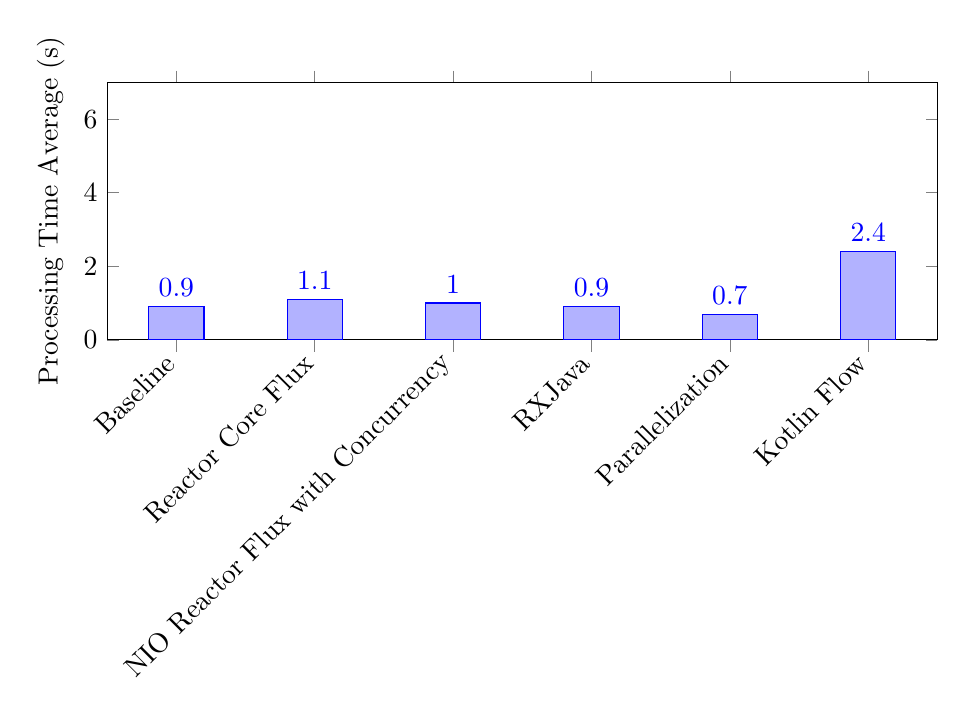
\begin{tikzpicture}
    \begin{axis}[
        ybar=2*\pgflinewidth,
        width=1.0\textwidth,
        height=0.4\textwidth,
        bar width=20pt,
        legend style={at={(0.5,-0.2)}, anchor=north, legend columns=-1},
        ylabel={Processing Time Average (s)},
        symbolic x coords={Baseline, Reactor Core Flux, NIO Reactor Flux with Concurrency, RXJava, Parallelization, Kotlin Flow},
        xtick=data,
        xticklabel style={rotate=45, anchor=east},
        nodes near coords,
        nodes near coords align={vertical},
        ymin=0, ymax=7,
        ]
    \addplot coordinates {(Baseline, 0.9) (Reactor Core Flux, 1.1) (NIO Reactor Flux with Concurrency, 1.0) (RXJava, 0.9) (Parallelization, 0.7) (Kotlin Flow, 2.4)};
    \end{axis}
    \end{tikzpicture}
    \caption{Processing times for different Java/Kotlin strategies for "Biggest Word".}
    \label{fig:biggest_word_processing_times_java}
\end{figure}
    
The Baseline, representing basic non-blocking I/O operations, provides a competent performance. Reactor Core Flux, utilizing the Project Reactor library for reactive programming, shows a processing time of 1.1 seconds, indicating slight overhead due to managing reactive streams. Enhancing Reactor Core Flux with concurrency reduces the processing time, demonstrating improved efficiency.
RxJava matches the baseline performance, indicating that does not introduce significant overhead. The most notable efficiency is achieved by the Parallelization strategy, which uses Java's Streams API with parallel processing using multithreading mechanisms, resulting in the fastest processing time. This highlights the advantages of parallel processing in optimizing computational tasks by distributing work across multiple threads.
On the other hand, Kotlin Flow, which employs Kotlin's Flow API for managing data asynchronously, shows the highest processing time, the overhead suggests potential areas for optimization.
These results highlight that parallel processing strategies although using blocking IO as a source, achieve the most efficient performance however, using non-blocking IO with reactive stream technologies like RXJava have a very good performance and its code is a loot simpler and easy to maintain than other solutions. This enforces that the chose between solutions are much dependent of the specific needs of the project.
However, we can see a huge difference from what we observed previously in .NET, where the baseline, parallelization, and Rx approaches showed significant differences in performance between each other, while in Java, the differences were minimal and their performances were orders of magnitude better than what we saw in .NET. The only performance that was similar in both JAVA and .NET was the performance related to parallelization using blocking IO, but even then, JAVA outperformed in 2 times the performance time of the .NET Implementation.
This reinforces the idea that choosing the right environment can have a much greater impact on project decisions than initially thought.

    \subsection{Group Word Results}
    \label{subsubsec:group_word_results}
    
   The strategies discussed here include:
    \begin{itemize}
        \item \textbf{Baseline}: This strategy serves as a baseline for comparison. It illustrates a basic non-blocking I/O operation without the use of any high-level constructs like Reactor Flux or Observable.
        \item \textbf{RXJava}: This strategy employs the RXJava library, popular for building asynchronous and event-driven applications.
        \item \textbf{Reactor Core Flux}: This strategy leverages the Reactor Flux model available in Java's Project Reactor library, providing an efficient approach to handling asynchronous data sequences.
        \item \textbf{Parallel}: This strategy uses Java's Streams API with blocking IO source and explores handling of blocking operations with the help of threadpools.
        \item \textbf{Streams}: This strategy uses Java's Streams API with blocking IO but without use of parallelization
        \item \textbf{Flow (Kotlin)}: This strategy utilizes Kotlin's Flow API
    \end{itemize}

    In the following table and graphic, we have the results in seconds for each strategy:
    \begin{figure}[H]
        \centering
        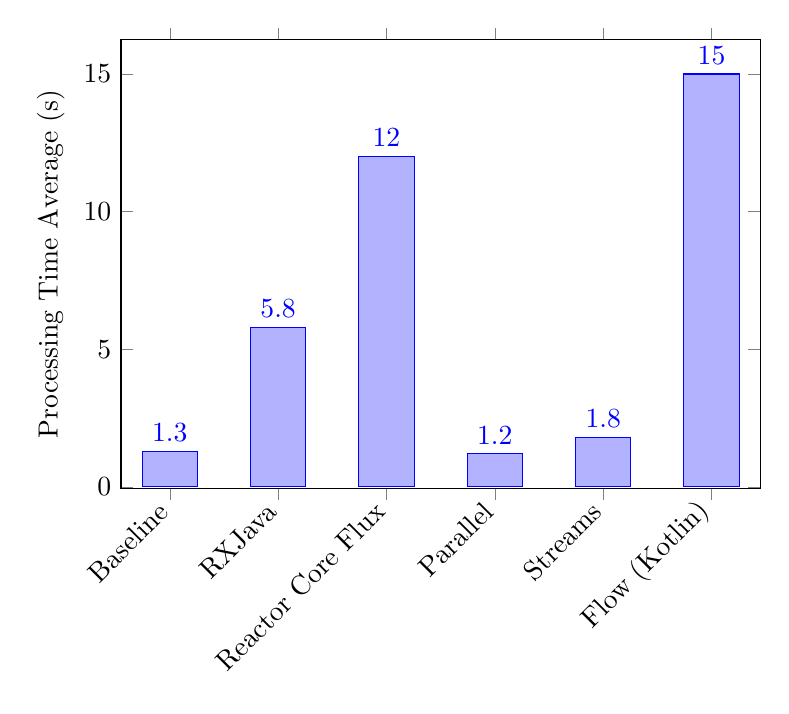
\begin{tikzpicture}
        \begin{axis}[
            ybar=2*\pgflinewidth,
            width=0.8\textwidth,
            height=0.6\textwidth,
            bar width=20pt,
            enlarge x limits={0.09}, % Adjust the value as needed
            enlarge y limits={0.09}, % Ensure only x-limits are enlarged
            legend style={at={(0.5,-0.2)}, anchor=north, legend columns=-1},
            ylabel={Processing Time Average (s)},
            symbolic x coords={Baseline, RXJava, Reactor Core Flux, Parallel, Streams, Flow (Kotlin)},
            xtick=data,
            xticklabel style={rotate=45, anchor=east},
            nodes near coords,
            nodes near coords align={vertical},
            ]
            \addplot coordinates {(Baseline, 1.3) (RXJava, 5.8) (Reactor Core Flux, 12.0) (Parallel, 1.2) (Streams, 1.8) (Flow (Kotlin), 15.0)};
        \end{axis}
        \end{tikzpicture}
        \caption{Processing times for different Java/Kotlin strategies for "Group Words".}
        \label{fig:group_word_processing_times_java}
    \end{figure}
    
    The Baseline strategy, as before, sets a standard for comparison, showing moderate efficiency. RXJava, known for its asynchronous and event-driven capabilities, demonstrates a longer processing time in this context, indicating potential overheads in handling complex data sequences in this particular environment. Reactor Core Flux, while efficient in handling asynchronous sequences, shows a significant processing time, possibly due to the complexity of the Group Word algorithm. Strategies involving parallel processing, whether through direct use of threadpools or the Streams API, exhibit improved efficiency, highlighting the benefits of parallelism in handling computationally and memory intensive tasks. Notably, Kotlin's Flow API, shows a longer processing time, which could reflect the overheads associated with its internal resource management in complex data processing scenarios.
    Overall to JAVA, these results illustrate the trade-offs between different programming paradigms and libraries in Java and Kotlin. 
    As we saw in "Find biggest word", we make again the observation of huge disparities between languages. In this case, although the "group words" algorithm having a similar implementation in both Java and .NET, the outcomes are significantly different between these two environments. For example, the baseline performance in .NET is in line with other approaches there, while in Java, the performance is significantly better compared to other approaches and also hugely outperforms the baseline in .NET.
    This reinforces the conclusion that underlying factors such as the programming language, virtual environment and runtime optimizations can have a substantial impact on the performance of systems, even when the algorithms are identical.

\section{JavaScript Benchmarking}
\label{sec:js_implementation}

In the case of the JavaScript solution, it is important to note that all I/O interactions were based on \texttt{fsPromises.readFile}, which is non-blocking I/O in nature. This function was used for both the reactive stream, streams and the baseline approaches.

\subsection{Finding the Biggest Word}
\label{subsec:biggest_word_js}

Here, we investigate the following three strategies:
\begin{itemize}
    \item \textbf{Baseline}: This strategy serves as the basic JavaScript approach for finding the biggest word, acting as a baseline for comparison.
    \item \textbf{Stream}: This strategy uses JavaScript streams, which provide a way to handle reading/writing files, network communications, or any kind of end-to-end information exchange in an efficient manner.
    \item \textbf{RxJS}: This strategy leverages the Reactive Extensions for JavaScript (RxJS) library, which offers a set of methods for dealing with asynchronous data sequences in an effective way.
\end{itemize}

In the following graphic, we have the results in seconds for each strategy:
\begin{figure}[H]
    \centering
    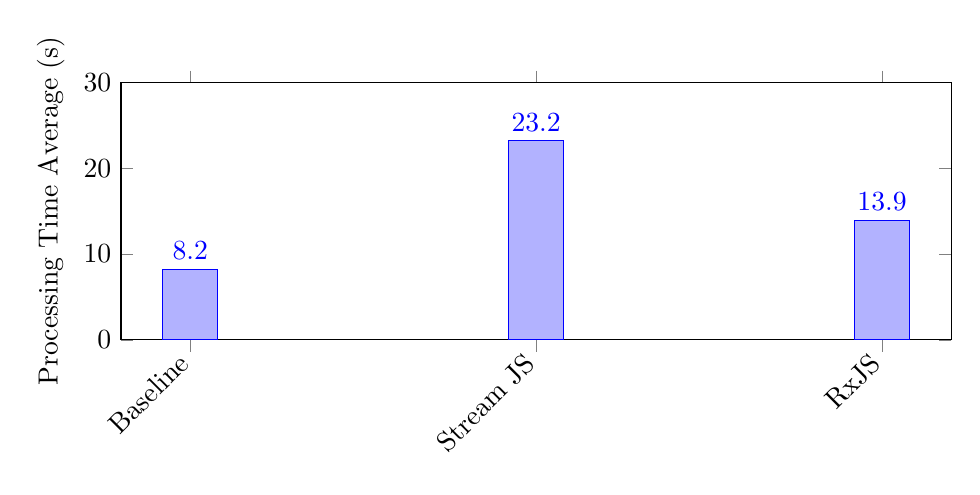
\begin{tikzpicture}
    \begin{axis}[
        ybar=2*\pgflinewidth,
        width=1.0\textwidth,
        height=0.4\textwidth,
        bar width=20pt,
        legend style={at={(0.5,-0.2)}, anchor=north, legend columns=-1},
        ylabel={Processing Time Average (s)},
        symbolic x coords={Baseline, Stream JS, RxJS},
        xtick=data,
        xticklabel style={rotate=45, anchor=east},
        nodes near coords,
        nodes near coords align={vertical},
        ymin=0, ymax=30,
        ]
    \addplot coordinates {(Baseline, 8.2) (Stream JS, 23.2) (RxJS, 13.9)};
    \end{axis}
    \end{tikzpicture}
    \caption{Processing times for different JavaScript strategies for "Find the Biggest Word"}
    \label{fig:biggest_word_processing_times_js}
\end{figure}

As we can see in this javascript implementation, the performance for "Find the Biggest" word algorithm of the baseline haves the best performance among its alternatives. On the other side, the algorithm implemented using RXJS library behaves slightly better than the alternative that makes use of JS streams API.
Once again, It's possible to see a difference between results in similar circumstances in different languages. In "Find biggest word" algorithm, the performance have a huge variance between languages. However, It's possible to see a pattern, that, baseline approaches have the tendency have better performance and some reactive stream solutions underperforms.
\subsection{Grouping Words}
\label{subsec:grouping_words_js}

In this subsection, we evaluate the following strategies for grouping words:

\begin{itemize}
    \item \textbf{Baseline}: This strategy serves as the basic JavaScript approach for grouping words, acting as a baseline for comparison.
    \item \textbf{Stream JS}: This strategy uses JavaScript streams, which provide a way to handle reading/writing files, network communications, or any kind of end-to-end information exchange in an efficient manner.
    \item \textbf{RxJS}: This strategy leverages the Reactive Extensions for JavaScript (RxJS) library, which offers a set of methods for dealing with asynchronous data sequences in an effective way.
\end{itemize}

In the following graphic, we present the results in seconds for each strategy: 

\begin{figure}[H]
    \centering
    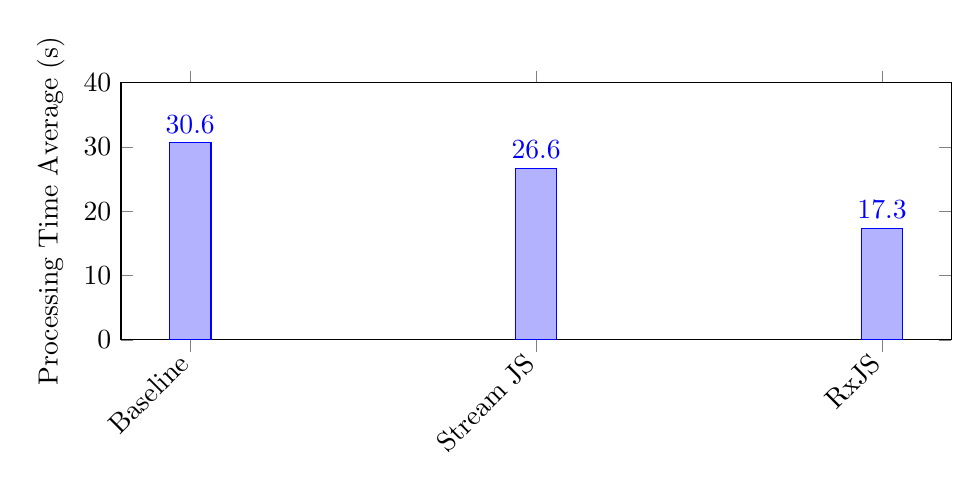
\begin{tikzpicture}
    \begin{axis}[
        ybar=2*\pgflinewidth,
        width=1.0\textwidth,
        height=0.4\textwidth,
        bar width=15pt,
        legend style={at={(0.5,-0.2)}, anchor=north, legend columns=-1},
        ylabel={Processing Time Average (s)},
        symbolic x coords={Baseline, Stream JS, RxJS},
        xtick=data,
        xticklabel style={rotate=45, anchor=east},
        nodes near coords,
        nodes near coords align={vertical},
        ymin=0, ymax=40,
        ]
    \addplot coordinates {(Baseline, 30.6) (Stream JS, 26.6) (RxJS, 17.3)};
    \end{axis}
    \end{tikzpicture}
    \caption{Processing times for different JavaScript strategies for "Grouping Words"}
    \label{fig:grouping_words_processing_times_js}
\end{figure}

In this case, the performance of the algorithms changes radically from what we observed with the "Group words" algorithm in other languages. Here, the baseline has the worst performance among the three strategies, while the RxStrategy has the best performance.
In other languages, the baseline approach tended to outperform or be in line with the reactive stream counterparts; however, in this case, that did not happen.
One explanation for these results is that the pipeline instructions in this case are optimized for managing large data containers, whereas the baseline approach is not. Additionally, these results highlight that performance can vary significantly between languages, frameworks, and virtual machines in similar algorithms.